\subsection{Application challenges}
\label{subsec: Application challenges}
As said before flexible PCBs offer great design flexibility and the possibility of implementing innovative designs and devices but they also come with their own set of \textbf{challenges}; especially in the case of flexible coils.

\subsubsection{Rise of high resistance}
Taking as an example the flexible coil we'll be using in our project, the resistance of the coil is about 30\(\Omega\). This is a relatively \textbf{high resistance} for such a small coil, especially when compared to traditional copper wire ones. 
This is due to the intrinsic structure of PCBs, especially flexible ones.
PCBs are created by etching very \textbf{thin copper traces} on a substrate, in the case of flexible PCBs, as the substrate must be flexible, their \textbf{thickness is even lower} and consequently also the traces are.

\begin{samepage}
    The coil can be considered as a very long strand of a very thin copper so its resistance can be calculated using the Ohm Law
    \begin{equation*}
        R=\rho \cdot \frac{L}{A}
    \end{equation*}
    \nopagebreak

    Where:
    \begin{itemize}
        \item \( R \) is the resistance [\(\Omega\)].
        \item \( \rho \) is the resistivity of the material [\(\Omega \cdot m\)].
        \item \( L \) is the length of the conductor [m].
        \item \( A \) is the cross-sectional area of the conductor [m\(^2\)].
    \end{itemize}
\end{samepage}

\begin{samepage}
    Then to find the length of the copper traces we can use the approximated formula \cite{Length_of_a_Spiral}
    \begin{equation*}
        L = N \pi \frac{D+d}{2}
    \end{equation*}
    \nopagebreak 

    Where:
    \begin{itemize}
        \item \( N \) is the number of turns.
        \item \( D \) is the outer diameter of the coil [m].
        \item \( d \) is the inner diameter of the coil [m].
    \end{itemize}
\end{samepage}

\begin{samepage}
    The tracks' cross-section is a \textbf{rectangle} so the area can be calculated as
    \begin{equation*}
        A = w \cdot t
    \end{equation*}
    \nopagebreak
        
    Where:
    \begin{itemize}
        \item \( w \) is the width of the track [m].
        \item \( t \) is the thickness of the copper [m].
    \end{itemize}
\end{samepage}

Finally considering the physical characteristics of our coil
\begin{table}[H]
    \centering
    \resizebox{.8\linewidth}{!}{
        \begin{tabular}{|l l|} % <-- Alignments: 1st column left, 2nd column left
    \hline
    \rowcolor{black} \multicolumn{2}{|c|}{\color{white} Coil Specifications} \cr
    \hline
    Track (width/spacing) & \quad $4/4mil = 1.016\cdot10^{-4}/1.016\cdot10^{-4}m$ \cr
    \hline
    Turns & \quad 2*35 (two coils in series) \cr
    \hline
    External radius & \quad $6.86\cdot10^{-3}m$ \cr
    \hline
    Copper thickness & \quad $0.5oz = 1.74\cdot10^{-5}m$ \cr
    \hline
    Resistivity & \quad $1.72\cdot10^{-8}\Omega m$\cr
    \hline
    Maximum Constant Power & \quad $0.8W$ \cr
    \hline
\end{tabular}
    }
    \caption{Physical characteristics of a Flexar coil}
    \label{tab: Physical characteristics of a Flexar coil}
\end{table}

The Length of the tracks (considering both spires) will be $L = 3.4548 m $ and the cross-section area will be $A = 1.7678e-09 m^2$.
As we can observe we have a wire that is both very long and very thin so a high resistance is expected (from the calculation $R = 33.61 \Omega $).

Also, the resistance of the coil is \textbf{dependent on the Temperature} of the coil, as the \textbf{temperature increases} the \textbf{resistance} of the copper \textbf{increases} as well. This is because the resistivity of copper increases with temperature. This is a problem as the coil releases a \textbf{lot of heat} when powered with \textbf{high currents}.

\begin{samepage}
    The temperature coefficient of resistivity of copper is $\alpha = 0.003862 \frac{1}{^{\circ}C}$ so the resistivity of copper at a certain temperature can be calculated as
    \nopagebreak

    \begin{equation*}
        \rho(T) = \rho_{T_{ref}} \cdot (1 + \alpha \cdot (T - T_{ref}))
    \end{equation*}
    \nopagebreak
        
    Where: 
    \begin{itemize}
        \item \( \rho_{T_{ref}} \) is the resistivity at the reference temperature [\(\Omega \cdot m\)].
        \item \( \alpha \) is the temperature coefficient of resistivity [\(\frac{1}{^{\circ}C}\)].
        \item \( T \) is the temperature [\(^{\circ}C\)].
        \item \( T_{ref} \) is the reference temperature [20 \(^{\circ}C\)].
    \end{itemize}
\end{samepage}
    
\begin{samepage}
    \subsubsection{Joule effect}
    \nopagebreak

    \label{subsubsec: Joule_effect}
    As said before, a coil of this type releases a lot of heat when powered with high currents. This is also due to its high resistance. 
    \nopagebreak

    The heat dissipated by a coil can be calculated using the formula
    \begin{equation*}
        P = I_{RMS}^2 R = \frac{V_{RMS}^2}{R}
    \end{equation*}
    \nopagebreak

    Where:
    \begin{itemize}
        \item \( P \) is the power dissipated by the coil [W].
        \item \( I_{RMS} \) is the root mean square current [A].
        \item \( V_{RMS} \) is the root mean square voltage [V].
        \item \( R \) is the resistance of the coil [\(\Omega\)].
    \end{itemize}
\end{samepage}

The coil can dissipate a maximum of 0.8W of power, this is a very low value and it is very easy to surpass it. This is a problem as the coil can be \textbf{damaged} if it dissipates more power than it can handle.

\begin{figure}[H]
    \centering
    \resizebox{0.5\textwidth}{!}{\begin{tikzpicture}
    \begin{axis}[
            xmin=0, ymin=0, xmax=8, ymax=2.5, samples=500,
            xlabel={Voltage [$V_{rms}$]},ylabel={Power [$W$]}, title={Power output vs $V_{rms}$}
        ]

        \addplot[blue, thick, domain=0:8, name path=func] (x, x^2/30);
        \addplot[red, thick, name path=limit] coordinates {
            (sqrt(0.8*30), \pgfkeysvalueof{/pgfplots/ymin}) 
            (sqrt(0.8*30), \pgfkeysvalueof{/pgfplots/ymax})
        }; % vertical limit line 

        \path[name path=axis] (axis cs:\pgfkeysvalueof{/pgfplots/xmin},0) -- (axis cs:\pgfkeysvalueof{/pgfplots/xmax},0);
        \path[name path=vend] (axis cs:\pgfkeysvalueof{/pgfplots/xmax},\pgfkeysvalueof{/pgfplots/ymin}) -- (axis cs:\pgfkeysvalueof{/pgfplots/xmax},\pgfkeysvalueof{/pgfplots/ymax});

        \addplot[red!25] fill between [of = limit and vend];
        % TODO: Add label to the limit line and legend
    \end{axis}
\end{tikzpicture}}
    \caption{Power profile of a Flexar coil}
    \label{fig: Flexar_power_profile}
\end{figure}

When exceeding the limit, even if the coil doesn't get damaged, the heat it releases can affect the \textbf{performance} of the coil. 
As the coil's resistance increases with temperature, the coil will dissipate even more power, this can lead to a \textbf{thermal runaway} situation where the coil will keep increasing its temperature until it gets damaged.
\nopagebreak

The only solution could be to introduce a \textbf{heat sink} to dissipate the heat but for the amount needed to be managed, heat sinks must be quite \textbf{bulky} and flexible solutions are not up to the task. %TODO: Aggiustare sta cazzo di scritta che se ne va a fanculo nella pagina dopo

\begin{samepage}
    \subsubsection{Magnetic field strength}
    As the coil can't be run at high currents, the \textbf{magnetic field} it generates will be \textbf{very weak}.
    \nopagebreak

    Considering the Flexar coil as an example we can plot the magnetic field strength, at the surface, as a function of the voltage applied to the coil using equation \ref{eq: Spiral_magn_field_eq} (considering the coil as a series of two spirals)
    \nopagebreak

    \begin{figure}[H]
        \centering
        \resizebox{0.5\textwidth}{!}{
            \begin{tikzpicture}
    \begin{axis}[
            xmin=0, ymin=0, xmax=8, ymax=8e-3, samples=500,
            xlabel={Voltage [$V_{rms}$]},ylabel={Magnetic Field [$T$]}, title={Magnetic Field vs $V_{rms}$}
        ]

        \addplot[blue, thick, domain=0:8, name path=func] (x, 9.14e-4*x);
        \addplot[red, thick, name path=limit] coordinates {
            (sqrt(0.8*30), \pgfkeysvalueof{/pgfplots/ymin}) 
            (sqrt(0.8*30), \pgfkeysvalueof{/pgfplots/ymax})
        }; % vertical limit line 

        \path[name path=axis] (axis cs:\pgfkeysvalueof{/pgfplots/xmin},0) -- (axis cs:\pgfkeysvalueof{/pgfplots/xmax},0);
        \path[name path=vend] (axis cs:\pgfkeysvalueof{/pgfplots/xmax},\pgfkeysvalueof{/pgfplots/ymin}) -- (axis cs:\pgfkeysvalueof{/pgfplots/xmax},\pgfkeysvalueof{/pgfplots/ymax});

        \addplot[red!25] fill between [of = limit and vend];
        % TODO: Add label to the limit line and legend
    \end{axis}
\end{tikzpicture}
        }
        \caption{Flexar magnetic field profile}
        \label{fig: Flexar_magnetic_field}
    \end{figure}
    \nopagebreak

    As we can observe even at the power limit of 0.8W ( $\simeq 5V$ ) the magnetic field generated by the coil is \textbf{very low} ( $\simeq 4mT$ ).
\end{samepage}

\subsubsection{Resistance parasitic effects due to AC current}
This paragraph will be a brief introduction to the \textbf{parasitic effects} that can occur in a coil due to the \textbf{AC current} that flows through it. All these effects are \textbf{negligible at low frequencies} (up to about 1kHz) which is the range we are aiming for in this project, but we will explore them for the sake of future research.

The main parasitic effects that can occur in a coil are:
\begin{itemize}
    \begin{samepage}
        \item \textbf{Reactance:} This is the opposition that a coil offers to the flow of AC current. This is due to the self-inductance of the coil which opposes the change in current flowing through it. This effect can lead to a change in the effective resistance of the coil.
        \nopagebreak

        The reactance of a coil can be calculated using the formula
        \begin{equation*}
            X_L = 2 \pi f L
        \end{equation*}
        \nopagebreak
            
        Where:
        \begin{itemize}
            \item \( X_L \) is the reactance of the coil [\(\Omega\)].
            \item \( f \) is the frequency of the AC current [Hz].
            \item \( L \) is the inductance of the coil [H].
        \end{itemize}
        \nopagebreak

        Then the impedance of the coil can be calculated as
        \begin{equation*}
            Z = \sqrt{R_{DC}^2 + X_L^2}
        \end{equation*}
    \end{samepage}

    \item \textbf{Skin effect:} This effect is due to the current flowing through a conductor tending to flow on the \textbf{surface} of the conductor. This gives rise to a \textbf{thin layer inside the conductor where all the current flows}. As a result, the effective resistance of the conductor \textbf{increases}. This effect is more pronounced at \textbf{higher frequencies}.
    
    \begin{figure}[H]
        \centering
        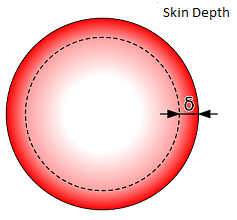
\includegraphics[width=0.4\linewidth]{Chapters/Chapter2/Flexible_PCB_coils/Figures/skin_depth.png} % TODO: Change image with svg
        \caption[Skin depth]{Representation of the thin surface generated by the skin effect}
        \label{fig: Skin_depth}
    \end{figure}

    \begin{samepage}
        The thickness of this area is called the \textbf{skin depth} and can be calculated using the formula
        \nopagebreak

        \begin{equation*}
            \delta = \sqrt{\frac{\rho}{\mu \pi f}}
        \end{equation*}
        \nopagebreak
                
        Where:
        \nopagebreak

        \begin{itemize}
            \item \( \delta \) is the skin depth [m].
            \item \( \rho \) is the resistivity of the conductor [\(\Omega \cdot m\)].
            \item \( \mu \) is the magnetic permeability of the medium [H/m].
        \end{itemize}
    \end{samepage}
    
    
    \begin{samepage}
        The effective resistance of the conductor can be derived from the skin depth using Dowell's equation \cite{AC_res_coils}
        \nopagebreak

        \begin{equation*}
            R_{skin} = F_{skin} \cdot R_{DC}
        \end{equation*}
        and
        \begin{equation*}
            F_{skin} = \frac{1}{2} (\frac{h}{\delta}) \frac{\sinh(\frac{h}{\delta}) + \sin(\frac{h}{\delta})}{\cosh(\frac{h}{\delta}) - \cos(\frac{h}{\delta})}
        \end{equation*}

        Where:
        \begin{itemize}
            \item \( R_{skin} \) is the effective resistance of the conductor due to the skin effect [\(\Omega\)].
            \item \( F_{skin} \) is the skin effect factor.
            \item \( h \) is the thickness of the conductor [m].
        \end{itemize}
    \end{samepage}

    \begin{samepage}
        In the case of the coil we're studying, the skin effect is \textbf{negligible} up to $1e8 Hz$ as the \textbf{thickness} of the flexible PCB's \textbf{traces} is \textbf{very low}.
        \nopagebreak

        \begin{figure}[H]
            \centering
            \includesvg[draft = false, width = 0.5\textwidth]{Chapters/Chapter2/Flexible_PCB_coils/Figures/Fskin_vs_freq.svg}
            \caption[Fskin of Flexar]{Logarithmic plot of the skin effect factor for a flexible PCB coil}
            \label{fig:Fskin of Flexar}
        \end{figure}
        \nopagebreak
    
        But we can observe from the study done on thicker traces' (0.5mm) coils that the skin effect starts to be already noticeable at $1e5 Hz$.
        \nopagebreak
        
        \begin{figure}[H]
            \centering
            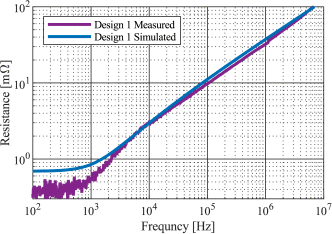
\includegraphics[width=0.5\columnwidth]{Chapters/Chapter2/Flexible_PCB_Coils/Figures/skin_effect_thicker.png}
            \caption[Skin effect on thicker traces]{Skin effect on thicker traces \cite{Sim_meas_AC_resistance_coils}}
            \label{fig: Skin_effect__thicker_trace}
        \end{figure}
    \end{samepage}

    \item \textbf{Proximity effect:} This effect is similar to the skin effect but it occurs when two conductors are close to each other. The current flowing through one conductor induces an \textbf{eddy current} in the other conductor which can lead to a change in the effective resistance of the conductors.
    
    \begin{figure}[H]
        \centering
        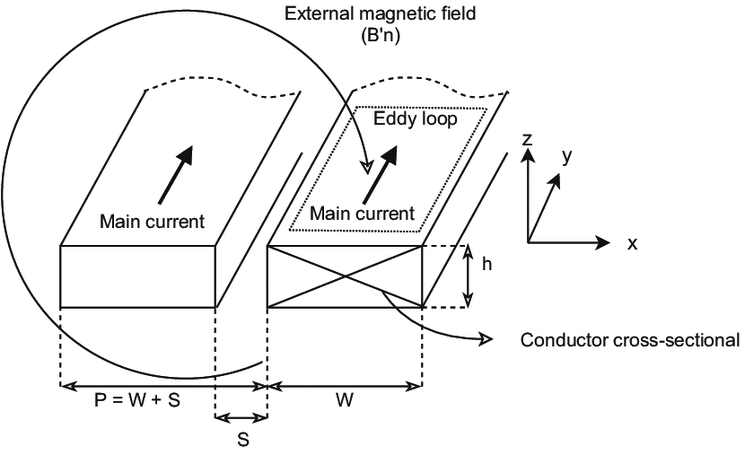
\includegraphics[width=0.8\columnwidth]{Chapters/Chapter2/Flexible_PCB_coils/Figures/proximity_effect.png}
        \caption[Proximity effect]{Representation of the proximity effect}
        \label{fig: Proximity_effect}
    \end{figure}

    \begin{samepage}
        The contribution of the proximity effect to the effective resistance of the coil can be calculated using the formula (considering current flowing in the coil $I_{ex} = 1A$) \cite{AC_res_Optimization}
        \nopagebreak

        \begin{equation*}
            R_{proximity} = \frac{1}{12} h \sigma \pi^2 f^2 B_n^2 w^3
        \end{equation*}
        \nopagebreak
        
        Where:
        \begin{itemize}
            \item \( \sigma \) is the conductivity of the conductor [\(\Omega^{-1} \cdot m^{-1}\)].
            \item \( h \) is the thickness of the conductor [m].
            \item \( f \) is the frequency of the AC current [Hz].
            \item \( B_n \) is the average external magnetic field [T].
            \item \( w \) is the width of the conductor [m].
        \end{itemize}
    \end{samepage}

    We can also approximate $F_{proximity}$ ($F_{proximity} = R_{proximity}/R_{DC}$) as
    \begin{equation*}
        F_{proximity} = \frac{F_{skin}}{3}
    \end{equation*}

    So when the contribution of the skin effect is negligible, the proximity effect will be \textbf{negligible} as well.

\end{itemize}





